%%
%% This is file `sample-sigconf.tex',
%% generated with the docstrip utility.
%%
%% The original source files were:
%%
%% samples.dtx  (with options: `sigconf')
%% 
%% IMPORTANT NOTICE:
%% 
%% For the copyright see the source file.
%% 
%% Any modified versions of this file must be renamed
%% with new filenames distinct from sample-sigconf.tex.
%% 
%% For distribution of the original source see the terms
%% for copying and modification in the file samples.dtx.
%% 
%% This generated file may be distributed as long as the
%% original source files, as listed above, are part of the
%% same distribution. (The sources need not necessarily be
%% in the same archive or directory.)
%%
%% The first command in your LaTeX source must be the \documentclass command.
\documentclass[sigconf]{acmart}
\usepackage{float}
\usepackage[inline]{enumitem}
\usepackage{tabularx}
\newcolumntype{C}{>{\centering\arraybackslash}X}
\usepackage{booktabs,array}
\usepackage{calc} % for calculating minipage widths
\usepackage{etoolbox}
\usepackage{siunitx}
\DeclareSIUnit\GHz{GHz}

\DeclareSIUnit\EiB{\exa{}iB}
\DeclareSIUnit\PiB{\peta{}iB}
\DeclareSIUnit\TiB{\tera{}iB}
\DeclareSIUnit\GiB{\giga{}iB}
\DeclareSIUnit\MiB{\mega{}iB}
\DeclareSIUnit\kiB{\kilo{}iB}
\DeclareSIUnit\EB{\exa{}B}
\DeclareSIUnit\PB{\peta{}B}
\DeclareSIUnit\TB{\tera{}B}
\DeclareSIUnit\GB{\giga{}B}
\DeclareSIUnit\MB{\mega{}B}
\DeclareSIUnit\kB{\kilo{}B}

\DeclareSIUnit\Eib{\exa{}ib}
\DeclareSIUnit\Pib{\peta{}ib}
\DeclareSIUnit\Tib{\tera{}ib}
\DeclareSIUnit\Gib{\giga{}ib}
\DeclareSIUnit\Mib{\mega{}ib}
\DeclareSIUnit\kib{\kilo{}ib}
\DeclareSIUnit\Eb{\exa{}b}
\DeclareSIUnit\Pb{\peta{}b}
\DeclareSIUnit\Tb{\tera{}b}
\DeclareSIUnit\Gb{\giga{}b}
\DeclareSIUnit\Mb{\mega{}b}
\DeclareSIUnit\kb{\kilo{}b}

\newcommand{\mytt}[1]{{\small\ttfamily\color{blue} \detokenize{#1}}}
\newcommand{\bgtt}[1]{\colorbox{black!05}{\small\ttfamily \detokenize{#1}}}
\newcommand{\mycode}[1]{\bgtt{\detokenize{#1}}}

\newcommand{\new}[1]{\textcolor{blue}{#1}}
\newcommand{\todo}[1]{\textcolor{red}{#1}}
\newcommand{\chck}[1]{\textcolor{red!70!yellow}{#1}}
\newcommand{\note}[1]{\textcolor{blue}{#1}}
\newcommand{\diff}[1]{\textcolor{green!70!black}{#1}}
\newcommand{\yell}[1]{\textcolor{magenta!70!black}{#1}}
\newcommand{\attn}[1]{\textcolor{magenta!70!black}{#1}}
\newcommand{\TODO}[1]{\textcolor{red}{{\bfseries #1}}}
\newcommand{\CHCK}[1]{\textcolor{red!70!yellow}{{\bfseries #1}}}
\newcommand{\NOTE}[1]{\textcolor{blue}{{\bfseries #1}}}
\newcommand{\DIFF}[1]{\textcolor{green!70!black}{{\bfseries #1}}}
\newcommand{\YELL}[1]{\textcolor{magenta!70!black}{{\bfseries #1}}}
\newcommand{\ATTN}[1]{\textcolor{magenta!70!black}{{\bfseries #1}}}

\newcommand{\highlight}[1]{\textcolor{magenta!70!black}{\bfseries #1}}

\newcommand{\supplement}[1]{\textcolor{magenta!70!black}{\small\ttfamily #1}}

\def\about{\textasciitilde}

\theoremstyle{plain}
\newtheorem{thm}{Theorem}[section]

%%
%% \BibTeX command to typeset BibTeX logo in the docs
\AtBeginDocument{%
  \providecommand\BibTeX{{%
    \normalfont B\kern-0.5em{\scshape i\kern-0.25em b}\kern-0.8em\TeX}}}

\begin{CCSXML}
<ccs2012>
   <concept>
       <concept_id>10003120.10003130</concept_id>
       <concept_desc>Human-centered computing~Collaborative and social computing</concept_desc>
       <concept_significance>300</concept_significance>
       </concept>
   <concept>
       <concept_id>10003456.10003462</concept_id>
       <concept_desc>Social and professional topics~Computing / technology policy</concept_desc>
       <concept_significance>300</concept_significance>
       </concept>
   <concept>
       <concept_id>10003456.10003457.10003580.10003584</concept_id>
       <concept_desc>Social and professional topics~Computing organizations</concept_desc>
       <concept_significance>500</concept_significance>
       </concept>
 </ccs2012>
\end{CCSXML}

\ccsdesc[300]{Human-centered computing~Collaborative and social computing}
\ccsdesc[300]{Social and professional topics~Computing / technology policy}
\ccsdesc[500]{Social and professional topics~Computing organizations}

%% Rights management information.  This information is sent to you
%% when you complete the rights form.  These commands have SAMPLE
%% values in them; it is your responsibility as an author to replace
%% the commands and values with those provided to you when you
%% complete the rights form.
\copyrightyear{2024}
\acmYear{2024}
\setcopyright{rightsretained}
\acmConference[PEARC '24]{\footnotesize Practice and Experience in Advanced Research Computing}{July 21--25, 2024}{Providence, RI, USA}
\acmBooktitle{\footnotesize Practice and Experience in Advanced Research Computing (PEARC '24), July 21-25, 2024, Providence, RI, USA}
\acmDOI{10.1145/3626203.3670602}
\acmISBN{979-8-4007-0419-2/24/07}

\usepackage{multirow}
%% The "author" command and its associated commands are used to define
%% the authors and their affiliations.
%% Of note is the shared affiliation of the first two authors, and the
%% "authornote" and "authornotemark" commands
%% used to denote shared contribution to the research.
\author{Becky Yeager}
\email{becky.yeager@colorado.edu}
\orcid{0009-0007-8526-9728}
\authornotemark[1]

\author{Shelley Knuth}
\email{shelley.knuth@colorado.edu}
\orcid{0000-0001-7249-4773}

\author{Alana Romanella}
\email{alana.romanella@colorado.edu}
\orcid{0000-0002-2309-0999}
\affiliation{%
  \institution{University of Colorado, Boulder}
  \streetaddress{Research Computing}
  \city{Boulder}
  \state{Colorado}
  \country{USA}
  \postcode{80303}
}

\author{Ben Nickell}
\email{ben.nickell@inl.gov}
\orcid{0000-0001-6352-9209}
\affiliation{%
  \institution{Idaho National Laboratory}
  \streetaddress{}
  \city{Idaho Falls}
  \state{Idaho}
  \country{USA}
  \postcode{83415}
}

\author{Chris Reidy}
\email{chrisreidy@arizona.edu}
\orcid{0000-0003-3565-1279}

\affiliation{%
  \institution{University of Arizona}
  \streetaddress{Research Computing}
  \city{Tucson}
  \state{Arizona}
  \country{USA}
  \postcode{85721}
}


\author{Jason Yalim}
\email{yalim@asu.edu}
\orcid{0000-0001-6866-9833}
\authornotemark[1]

\affiliation{%
  \institution{Arizona State University}
  \streetaddress{Research Technology Office}
  \city{Tempe}
  \state{Arizona}
  \country{USA}
  \postcode{85287}
}

\title[% short title
Identifying HPC needs in a regional consortium
]{% title
Identifying high-performance computing needs at member institutions in
a regional consortium
}

\keywords{%
HPC Consortia,
Democratization, 
Workforce Development%
}

\begin{document}

\begin{abstract}
The Rocky Mountain Advanced Computing Consortium (RMACC) is a
collaborative organization of academic, government, and professional
research institutions located throughout nine inter-mountain states.
RMACC's mission is to facilitate the efficient adoption of
high-performance computing (HPC) resources within the region.  During
the Summer of 2023, the Executive Committee of RMACC conducted
thirty-minute interviews with the majority of its thirty-four member
institutions. As a result of these interviews, several opportunities and
challenges in regional HPC practices were identified. Our findings
indicate the importance of strong connections between institutions to
enhance collaboration and support Research Computing regionally.
Specific themes indicate increased knowledge sharing, additional
networking opportunities, and opportunities for workforce development to
aid in technical staff retention and student growth.  A need for a
variety of training was specifically outlined, as well as additional
support for systems professionals who may be the only (or one of few)
supporting a cluster at their institution.
\end{abstract}

\maketitle

\vspace{-1em}
\section{Introduction and Background}
The Rocky Mountain Advanced Computing Consortium (RMACC) was founded in
2011 by Dr. Thomas Hauser, then Director of Research Computing at The
University of Colorado (CU) Boulder \cite{RMACC:web}. In the Fall of
2010 leadership at Front Range educational institutions and National
Labs in Colorado and Wyoming met to establish a committee to pursue
regional HPC collaboration opportunities. RMACC was officially
established in 2014 with expansion out to Utah, Montana, Idaho and New
Mexico, and grew from the success of the original Front Range Consortium
for Research Computing (FRCRC) which comprised Colorado State University
(CSU), CU Boulder, CO Sch.\ of Mines, U.\ of Wyoming, the National
Center for Atmospheric Research (NCAR), the National Renewable Energy
Laboratory (NREL), and the National Oceanic and Atmospheric
Administration (NOAA).  In 2018 RMACC expanded to include schools in
Nevada, Washington, and Arizona. 

RMACC has been successful in acquiring funding to support
under-resourced regional institutions and expand opportunities for
individuals. At the time of this writing, there have been six direct
National Science Foundation (NSF) awards directly supporting RMACC totaling
just over \$6 million, with NSF numbers:
1532235, 
1532236, 
1659425, 
1925766, 
and including two currently active NSF awards, 
2201538 \& 
2322260. 
The first two grants supported RMACC's Summit supercomputer, which
provided 85-million core-hours per year to RMACC members
\cite{RMACC:Summit:PEARC17}. The third resulted in the creation of the
RMACC ``Cyberteam'' in 2017 to provide cyberinfrastructure support for
members \cite{RMACC:CITeam:PEARC19,RMACC:CITeam:Survey:OSF19}.

\begin{figure*}[t]
\centering
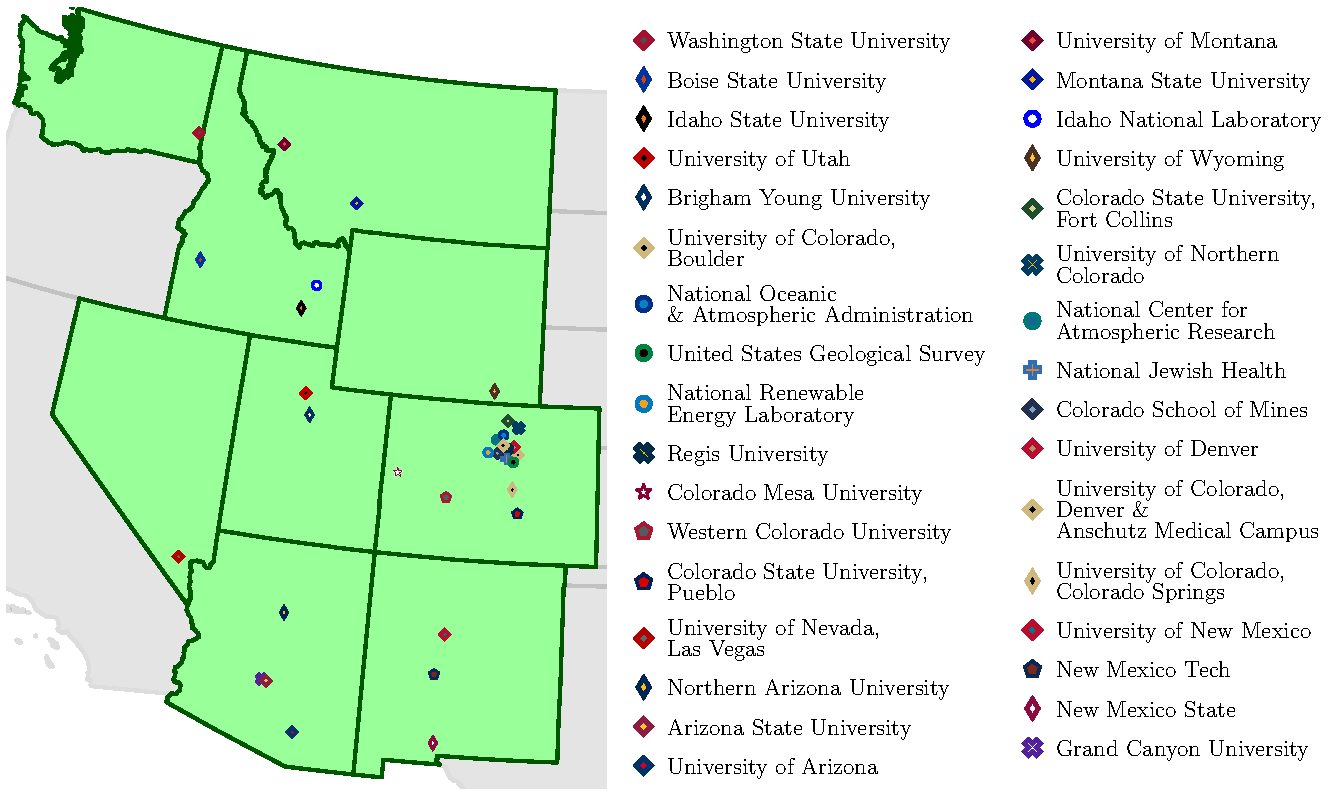
\includegraphics[width=1\linewidth]{figs/RMACC-members-with-legend.pdf}
\caption{%
  Map of the western continental United States with RMACC's thirty-four
  members' host states highlighted in green. Markers indicate the
  locations of participating RMACC institutions. Marker types indicate
  institution type, i.e., universities that are R1 (square diamonds), R2
  (rhombuses), D/PU (filled-X), M2 or M3 (pentagons), else (stars); the
  hospital (filled plus); the government entities (circles).  As
  illustrated, the five Denver, three Boulder, and two Golden locations
  in Colorado are shifted slightly from respective city centers to
  improve visibility. Note: University of Colorado Denver and Anschutz
  Medical Campus are distinct RMACC members.% 
}
\label{fig:members}
\end{figure*}

Despite the benefits that they provide, regional HPC Consortia are not
universal.  In 2009, Gropp \& Snir
\cite{IJHPCA_GrSn09:Call:HPC:Consortia} called for the creation of an
HPC consortium to improve the efficiency and software quality of HPC
systems, discussing unaddressed gaps in an ``[HPC] performance
pyramid.'' The authors specifically wanted an institutional-sharing
structure more focused than the existing nationwide consortia (like
TeraGrid) that could facilitate operational and end-user practice
sharing, as well as increase collaboration and increase software
homogeneity across centers.  There are a number of U.S.-scale consortia,
like Advanced Cyberinfrastructure Coordination Ecosystem: Services \&
Support (ACCESS), which replaced the Extreme Science and Engineering
Discovery Environment (XSEDE), which had replaced TeraGrid. ACCESS is
most comparable to Compute Canada or the international PaRtnership for
Advanced Computing in Europe (PRACE) \cite{JPCS12_Bal:ComputeCanada}.
In the United States, the National HPC Consortium was founded for
fighting COVID-19
\cite{CSE_HaPa20:HPCConsortium:COVID,CSE_BraseEtAl22:HPCConsortium:COVID},
demonstrating how networks of HPC centers can improve the state of the
art and decrease the time to science or, especially in the case of
COVID, help direct policy. There are a number of regional networks that
are more comparable to RMACC. These include but are not limited to
SWEETER, the NE Cyberteam, the Great Plains Network, and the ECEP
\cite{%
  SWEETER:web,SWEETER,
  NECyberteam:web,NECyberteam:A,NECyberteam:B,JCSE:NECyberteam:C,
  GPN:web,GPN06,
  ECEP:web,ECEP12%
}. In order to operate efficiently, consortia member needs must be
regularly assessed.

At the time of this writing, RMACC has thirty-four member institutions.
Figure~\ref{fig:members} illustrates where these member institutions are
with markers that reflect the 2021 Carnegie classifications
\cite{carnegie21:web} of academic members, or if a member is a hospital
or Federal Government entity. Twenty-eight of RMACC's members are
academic, and by the shorthand defined in the 2021 ``Basic
Classification'' Carnegie classifications
\cite{carnegieclassifications:basic:web}:
fourteen\footnote{%
The University of Colorado Anschutz Medical Campus is considered a
distinct RMACC member, but is combined with the University of Colorado
Denver in the Carnegie classifications.
} are R1, seven are R2, three are D/PU, two are M2, one is M3, and one
is ranked as a Baccalaureate College with Diverse Fields.  Five of
RMACC's members are Government entities:
NREL, NOAA, USGS, NCAR/UCAR, and INL. 
One of RMACC's members is a research hospital. 

RMACC's member institutions are often represented by their expert HPC
facilitators and researchers. To determine consortia members' needs, 
one-on-one, video-conferenced interviews with those representatives were
organized by RMACC's Executive Committee. The results from those
interviews and the resulting discussion of the Executive Committee are
qualitatively reported by this short paper.

\subsection{RMACC Structure and Benefits}
RMACC is a free collaborative network for computational researchers and
HPC facilitators to draw from and contribute to. The organization
maintains an enterprise Slack channel as a forum for member
communication. Funding typically comes from sponsorship and registration
for an annual HPC Symposium which is historically hosted in May by CU
Boulder. In 2023 it was hosted by Arizona State University (ASU); the
host is planned to start rotating annually among member sites by 2025.
The HPC Symposium has typically been a two-and-a-half day event,
primarily focused on encouraging presentations, discussions, and
collaborations between system administrators, facilitators, researchers,
and industry sponsors.  Attendees often will present site-updates and
discuss operational challenges and opportunities with one another. The
Symposium also encourages student participation by hosting a Student
Poster competition. The winner is awarded full financial support to
attend a larger global conference, typically SuperComputing. 

An annual system administrator meetup is organized by RMACC. It has
typically been hosted in August--October at a rotating host site, e.g.,
it was hosted by CSU in Fort Collins in 2023 over two-and-a-half days in
late September. 

RMACC is led by an Executive Committee, which is currently comprised of
six members. Community-wide elections select the Chair, Vice-Chair,
Executive Director, and three Board members by simple majority.
Elections take place every two to three years, the timing of which
balances the effort involved in conducting elections and maintaining
effective community representation. The Executive Committee meets at
least monthly to discuss and act upon the operation and needs of the
Consortium.

RMACC has three major subcommittees that focus on systems, users, and
Diversity, Equity, and Inclusion (DEI) topics. The three subcommittee
meetings occur at least monthly and are open to the broader community.
Ad hoc subcommittees will form and disband to organize and support the
annual HPC Symposium and system administrator meetup.

\section{Member Interviews}
Over August--October of 2023, Executive Director Becky Yeager met with
representatives from thirty-one of the thirty-four RMACC members. The
Executive Director was typically joined by one other RMACC Executive
Committee member to help facilitate the interview process. Member
institution representatives were typically HPC center leaders, system
administrators, or facilitators (see table~\ref{tab:interview}) ---
those who are the primary contacts for RMACC communications and often
participate in RMACC's events.  Each member was asked the same set of
questions, which are highlighted in figure~\ref{item:interview}.

Additionally, two interviews were conducted for the RMACC DEI
subcommittee by Executive Director Becky Yeager. These interviews were
conducted in a one-hour meeting and covered the same questions as the
member interviews with time to delve deeper into the answers and more
complex questions. 

Interview notes were collected in a shared Executive Committee document
and further discussed by the Executive Committee during regular
meetings. The qualitative analysis and inference from those discussions
form the basis of this report. 

\begin{table}[ht]
  \centering
  \begin{tabular}{rc}
    role & \# \\
    \hline
    HPC Director or CIO & 14+1  \\
    System Administrators & 14 \\
    User Facilitators & 8 \\
    Multiple Roles & 6+1 \\
    Faculty & 5 \\
    Other Role & 4 \\
    Researcher & 2 \\
    Student & 1 \\
    \hline
    \hline
    Total & 54+2
  \end{tabular}
  \caption{%
  Interviewee roles from the thirty-one conducted member interviews.
  The additional two interviewees were from a set of two interviews
  conducted for the RMACC DEI subcommittee by Executive Director Becky
  Yeager.%
  }
  \label{tab:interview}
\end{table}

\begin{figure}
  \begin{center}
%   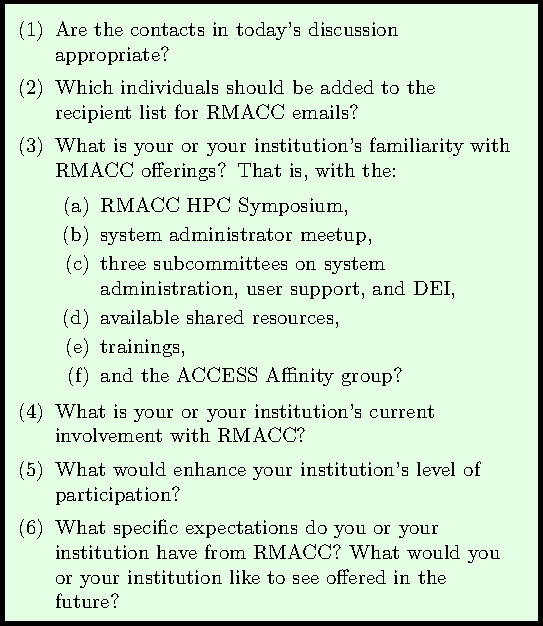
\includegraphics[width=1\linewidth]{figs/interview-questions-highlight.pdf}
    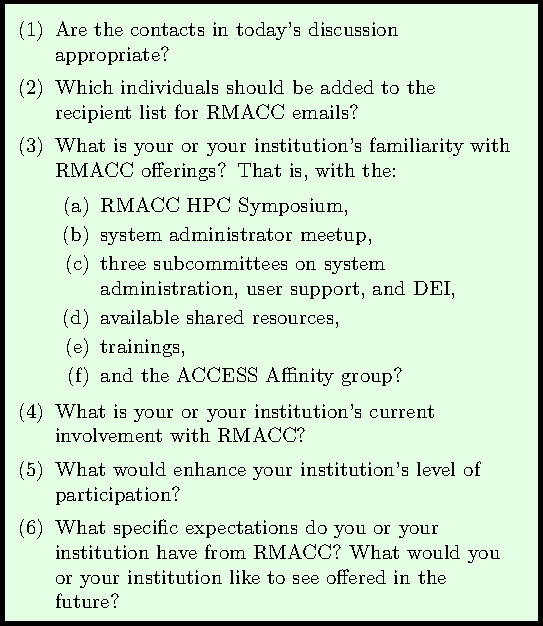
\includegraphics[width=8.5cm]{figs/interview-questions-highlight.pdf}
  \end{center}
  \caption{\label{item:interview}%
    List of interview questions, which were asked to each participating
    member.%
  }
\end{figure}

\subsection{Interview Findings}

Nineteen member institutions reported having on-premise computational
resources, with eleven members relying on RMACC or National (ACCESS)
resources for research computing needs.

There were a number of overarching themes and requests. The interviewees
all communicated a need for more:
\begin{enumerate}%[label={\arabic*.)}]
  \item
  training for the users of member HPC systems as well as for the
  faculty and staff supporting those users,
  \item
  knowledge sharing between RMACC partners about topics of interest to
  their staff, e.g., effective grant writing, or their users, e.g.,
  application affinity groups,
  \item
  networking opportunities and chances to gather with their regional
  peers to discuss topics of interest,
  \item
  hardware resource sharing within the region,
  \item
  and an improved ability to discover available resources both
  regionally and nationally.
\end{enumerate}

As a result of the interviews, several immediate actions were taken. To
improve inter-institutional transparency and facilitate collaboration, a
Google spreadsheet was shared among member institutions. This
spreadsheet had two subsheets that members were asked to fill out. The
first sheet was for self-reporting site information, collaboration
goals, and RMACC-sharable resources (e.g., the University of Colorado
Boulder's Alpine). The second sheet collected information on member
institutions' flagship system, storage options, personnel, and service
offerings, such as cloud or secure compute. 

To help facilitate outreach, networking, and educational opportunities
for system administrators, the existing sysadmin group will be brought
more formally under the RMACC umbrella. This includes ensuring that the
main HPC symposium has a dedicated sysadmin track for its entire
duration.  Additionally, the group's monthly meeting will be more
formalized with pre-cultivated conversation topics that encourage those
facilitation goals.  The other RMACC communities will also adopt this
structure. Additionally, opportunities for the community to gather at
external conferences, i.e., SuperComputing and PEARC, will be organized.

To address member interests, a more regular cadence of community
conversations will be developed, on topics including grants, ACCESS, and
available resources for RMACC members. Opportunities for member
lightning talks will be provided.

A committee was created to develop a list of more ``generic" trainings
that are not institution or machine-specific and can be offered remotely
or asynchronously to enable attendance by the RMACC community. One of
the synchronous goals is to create a calendar of shared trainings on the
RMACC website, as well as a collated list of shared training resources
on the RMACC web site. This list includes documentation, training
videos, and other available resources from RMACC members. This list will
be made available to the ACCESS Knowledge Base.

A plan is in place to meet with smaller RMACC member institutions to
learn about their needs regarding the use of the RMACC partition on the
Alpine Supercomputer and develop specific trainings from the University
of Colorado Boulder that meet their specific needs and questions. 

Finally, in part due the interviews conducted by RMACC, the ACCESS
project has put out a call to fund community-led workshops on workforce
development.

\section{Discussion and Next Steps}

There is a training gap on how to administer new systems.
Under-resourced institutions would especially benefit from better
information sharing on how to obtain funding for new systems, as well
as how to train personnel, set-up, administer, and support users on
said system. Topics range from, for example, working with a scheduler
or debugging MPI on multi-node systems. 

Correspondingly, there are higher-education training gaps for students
interested in HPC careers, including a lack of clear degree programs
paths or the courses that appropriately foster expertise, like in
systems administration or user support.  Many of the smaller
institutions need workers who have the ability to support users and
conduct system administration. This is driven by a general lack of
personnel as well as funding for additional hires.  Because of the
lack of training and workforce development the number of trained
administrators does not meet the regional demand and need for trained
administrators. These roles are being filled by faculty and staff who
do not have the technical expertise needed to fill the gaps, resulting
in split time between research, teaching classes, administering and
building systems, and supporting others in their research without
formal training in those areas. 

Training opportunities are further challenged by DEI issues; there are
no quick pathways to a successful career. Issues of equity and
inclusion in rural areas are a challenge as other career paths are more
visible and readily available for students. With a lack of training
and workforce development many students are not aware of the
opportunities that exist. 

Remote areas have additional difficulty in recruiting talent.  With a
small pool of available HPC-trained workers and open positions at
larger R1 institutions available it is difficult to find employees who
are interested and willing to live in remote areas. Smaller
institutions find it difficult to compete for the available pool of
workers because of challenges with pay scales, location, and skill set
needed. 

Finally, it is difficult to find resources to learn on.  While there
are many national resources available for researchers and users, there
is a general gap in the communication of the existence of those
resources and how to access them. Additionally, when training
materials do exist, often they are provided at an expert level, making
assumptions that new users will have a basic understanding
of a command-line interface, which is not always the case.  Training
to both find the resources and use them, would benefit these 
schools that do not have their own trainers or user documentation.

Taken together, many institutions are limited in their ability to move
up the pyramidal HPC hierarchy of needs, but directed organizational
efforts, particularly with funding, can increase the research
efficiency and agency of smaller member institutions in ways that may
be replicated to the wider national community.  While RMACC may not be
able to solve all of these issues, it has spurred a number of ideas
that are in the early stages of development.  

One such effort involves working with the ACCESS project to
decentralize their outreach efforts.  In part due to these findings,
ACCESS is in the late stages of developing a campaign to support
individuals' attendance at conferences in return for assistance with
developing materials on their resources.  This will allow the material
provided on ACCESS resources and activities to be provided in
community members' own words, which will enhance knowledge sharing.
Several RMACC partners are also in the very early stages of developing
a plan for a program that will provide both formal and informal
training in HPC systems, storage, and network administration.
Additionally, several RMACC members have partnered together as part of
OAC grant no.\ 2322260 to form a cohort of student undergraduates who
are working closely with system administrators employed at CU Boulder
to engage in hands-on work to design, procure, and deploy new hardware
for the Alpine cluster.

\section{Conclusion}

Our findings highlight a need within the RMACC community to bolster
collaboration and support among member institutions. By implementing
strategies such as information exchange opportunities, formalizing
sysadmin groups, and organizing regular meetings with curated topics,
the RMACC community aims to foster networking, knowledge-sharing, and
educational opportunities. As a regional organization, initiatives such
as remote training opportunities and tailored support for smaller
institutions demonstrate a commitment to inclusivity and addressing the
diverse needs of the region while also promoting the regional adoption
of HPC/CI. Moving forward, these efforts are poised to strengthen the
relationships between RMACC members, promote innovation, and enhance the
overall effectiveness of collaborative endeavors within the research
computing landscape. 

\begin{acks}
This work is supported by the National Science Foundation under Grant
Numbers 2138286 and 2322260. This research was also supported by Idaho National
Laboratory's High Performance Computing located at the
Collaborative Computing Center and supported by the Office of Nuclear
Energy of the U.S. Department of Energy and the Nuclear Science User
Facilities under Contract No.\ DE-AC07-05ID14517.  
\end{acks}

%\appendix

%\bibliographystyle{unsrt}
\bibliographystyle{ACM-Reference-Format}
\bibliography{references.bib}

\end{document}
\endinput
